Все рассмотренные в предыдущем разделе методы перестроения поверхностей объединяет одно сходство -- они сохраняют количество элементов расчетной сетки (узлы, ребра, грани) и связи между ними.
Несмотря на некоторые специальные методы по предотвращению конфликтов между гранями сетки и методы сглаживания, после формирования новой поверхности возможно возникновение самопересечений, появление граней неправильной формы, а также неравномерное распределение граней в сетке по размеру.
Пока опустим самопересечения сетки и будем рассматривать только вопросы, касающиеся формы и размера ячеек.

\begin{figure}[h]
  \centering
  \begin{minipage}[h]{0.35\textwidth}
    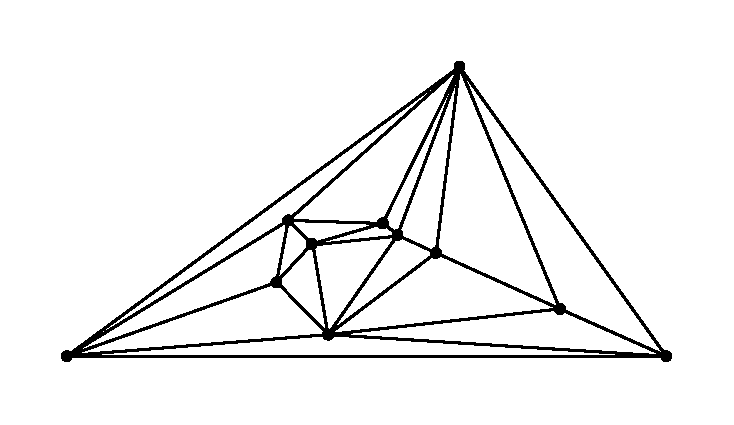
\includegraphics[width=\textwidth]{pics/pic_delaunay_size.pdf}
    \caption{Разбиение ячейки с помощью триангуляции Делоне.}\label{fig:pic_delaunay}
  \end{minipage}
  \hfill
  \begin{minipage}[h]{0.35\textwidth}
    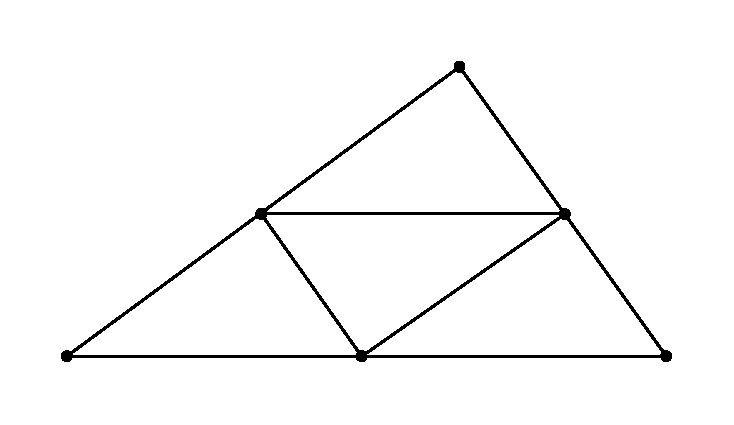
\includegraphics[width=\textwidth]{pics/pic_delaunay_2_size.pdf}
    \caption{Дробление ячейки на более мелкие.}\label{fig:pic_delaunay_2}
  \end{minipage}
  \hfill
  \begin{minipage}[h]{0.28\textwidth}
    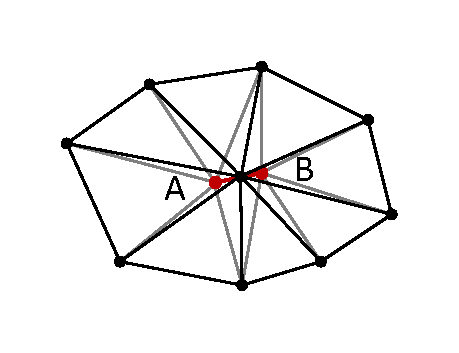
\includegraphics[width=\textwidth]{pics/pic_reduce_edge_size.pdf}
    \caption{Стягивание ребра.}\label{fig:pic_reduce_edge}
  \end{minipage}
\end{figure}

Первая операция, которая нам потребуется -- разбиение ячейки на более мелкие.
Во всех случаях будем выполнять разбиение ячеек с помощью триангуляции Делоне, считая что для разбиения нам известен набор точек внутри разбиваемой ячейки (Fig.~\ref{fig:pic_delaunay}) \cite{Rivara}.
Стоит отметить, что разбиение ячейки можно производить с сохранением локальной кривизны сетки, как это показано в \cite{Rakotoarivelo}, но для простоты будем производить разбиение исключительно в плоскости ячейки.
Если точка разбиения находится не внутри ячейки, а на ее ребре, то разбить придется также вторую инцидентную ячейку этого ребра (рассматриваются только сетки, ребра которых имеют ровно по две инцидентные ячейки, как это указано в (\ref{eq_arch}).
Иногда для уменьшения размера требуется просто разбить ячейку на более мелкие без задания точек разбиения.
В этом случае необходимо следить за качеством результирующих ячеек.
Для определения качества формы ячейки треугольной формы с узлами $\vec{A}$, $\vec{B}$, $\vec{C}$ можно пользоваться простым критерием качества

\begin{equation}
Q(f) = \frac{4\sqrt{3} S_{ABC}}{|\vec{AB}|^2 + |\vec{BC}|^2 + |\vec{AC}|^2}
\end{equation}

где $Q(f) = 1$ соответствует идеальному случаю равносторонней ячейки, а $Q(f) = 0$ -- худший случай для ячеек с нулевой площадью \cite{Borouchaki}.
Для выполнения разбиения ячейки на более мелкие с сохранением их качества просто выполним разбиение по серединам всех ее сторон (Fig.~\ref{fig:pic_delaunay_2}).

Вторая операция, которая необходима для адаптации сетки, связана с огрублением.
Достаточно часто во время выполнения триангуляции по множеству заданных точек могут появляться ячейки с низким показателем качества (у них могут присутствовать либо слишком острые углы, либо близкий к развернутому угол).
Если в ячейке присутствует угол, близкий к развернутому, то избавиться от него поможет разбиение по наибольшей стороне (при этом в качестве точки разбиения следует выбрать основание высоты, опущенной из противолежащего узла).
Если же в треугольнике присутствуют лишь близкие к острым углы, то значит в нем есть слишком короткая сторона, которая может быть удалена.
При удалении ребра $AB$ удаляются обе инцидентные ей грани, узлы $A$ и $B$ соединяются в единый узел $A'$, а все ребра из множества $\mathscr{E}(A) \cup \mathscr{E}(B)$ перенаправляются на узел $A'$ с учетом удаления повторных (Fig.~\ref{fig:pic_reduce_edge}).
Данную операцию будем называть стягиванием ребра \cite{Panchal}.
Путем применения стягивания наиболее коротких ребер в расчетной сетке можно добиться произвольной степени огрубления.
